\section{问题定义}
\label{sec:problem}

本文对构造原则与学习者能力的共演化进行形式化描述，并将其中的课程分配建模为序贯决策问题。在第 $e$ 轮，分配向量 $\boldsymbol q_e$ 规定有限构造预算在各任务内预先定义的能力单元之间的分配比例，并满足固定的任务级配额约束。构造原则 $\Sigma_e$ 是决定如何将医学证据组织为面向目标能力的监督的可复用规范。这些原则明确问题意图，指导回答如何依据医学证据形成，并厘清概念区别。

\subsection{学习者状态与课程分配}

第$e$轮的学习者$M_e$在独立任务验证集$\mathcal V=\{\mathcal V_t\}_{t\in\mathcal T}$上接受评价，其中$\mathcal T$为验证任务集合。支持集$\mathcal S$提供监督构造所需的医学视觉证据及关联文本，独立外部基准评价泛化。预先定义的能力单元组成$\mathcal C$，每个单元$c$在固定非空子集$\mathcal V_c\subseteq\mathcal V_t$上接受评价。能力评价泛函$\mathcal J_c$将预测行为映射为实测掌握水平：
\begin{equation}
\mathcal J_c[M_e]=\frac{1}{|\mathcal V_c|}\sum_{z\in\mathcal V_c}u_c(M_e,z),
\qquad
\widehat{\boldsymbol\kappa}_e=\bigl(\mathcal J_c[M_e]\bigr)_{c\in\mathcal C}.
\label{eq:capability_level}
\end{equation}
其中，$u_c$为对每个样本赋予分数的固定评价规则，分数越高表示表现越好。向量$\widehat{\boldsymbol\kappa}_e$为可观测能力表征。任务表现与错误证据共同构成观测$o_e$。

课程规划器依据历史摘要$\mathbf{s}_e=\Phi(h_e)$选择课程动作$a_e$，其中$h_e$记录截至第$e$轮的观测、动作与奖励。我们以有限时域部分可观测马尔可夫决策过程刻画这一交互~\citep{kaelbling1998planning,matiisen2017teacher}。完整状态$X_e$包含学习者参数与优化状态、生效构造原则、修订历史、调度信息及剩余资源。给定原则演化规则$\mathscr E$，有
\begin{equation}
P(X_{e+1}\mid X_{0:e},a_{0:e})
=P_{\mathscr E}(X_{e+1}\mid X_e,a_e).
\label{eq:transition}
\end{equation}
转移包括监督构造、验证、学习者更新及学习响应驱动的原则修订。附录~\ref{app:formalization}给出完整状态与观测模型。

\subsection{监督构造}
\label{sec:supervision_evolution}

对于由视觉输入、指令与目标回答组成的$z=(v,x,y)$，候选训练样本的分布为
\begin{equation}
\widetilde p_e(z)=\sum_{c\in\mathcal C}q_{e,c}\,
g_{e,c}(z;\Sigma_e,\mathcal S).
\label{eq:supervision_mixture}
\end{equation}
其中，$g_{e,c}$表示第$e$轮面向能力单元$c$的候选训练样本在验证前的概率分布，由构造原则$\Sigma_e$指导、利用支持集$\mathcal S$开展的证据选择与监督构造过程诱导。非负份额$q_{e,c}$的总和为1。原则演化改变各分量的监督内容，课程分配改变其相对投入。证据约束的验证形成接受的监督$\mathcal D_e^{\mathrm{syn}}$，后续混合确定实际训练曝光。

\subsection{学习者更新与策略目标}

训练混合数据$\mathcal D_e^{\mathrm{mix}}$由已接受的监督$\mathcal D_e^{\mathrm{syn}}$与允许使用且仅用于训练的原始或回放数据$\mathcal R_e$组成。学习者更新为
\begin{equation}
M_{e+1}=\mathcal U(M_e,\mathcal D_e^{\mathrm{mix}}),
\label{eq:learning_dynamics}
\end{equation}
其中，$\mathcal U$遵循规定训练协议及优化状态。各轮能力表征记录$E$轮训练中的学习者能力发展。$M_{e+1}$的响应进入$h_{e+1}$，并通过式~\ref{eq:strategy_evolution}修订$\Sigma_{e+1}$，将原则演化与后续学习相联系。

在这一动态中，分配策略最大化累积验证学习进展：
\begin{equation}
\max_{\pi\in\Pi_{\mathrm{adm}}}
\E_{\pi}\left[\sum_{e=0}^{E-1}\gamma^e r_e\right],
\label{eq:objective}
\end{equation}
其中，$\Pi_{\mathrm{adm}}$表示满足构造预算约束并保持各任务规定配额的课程分配策略集合，$\gamma\in[0,1]$为折扣因子。奖励$r_e$衡量对 VQA 与报告生成赋予相同权重的验证表现增益（第~\ref{sec:curriculum}节）。附录~\ref{app:cumulative_gains}给出累积增益与各轮学习表现之间的关系。

\FloatBarrier

\section{CoEvoMed：监督构造智能体与多模态学习者的共演化}
\label{sec:method}

\begingroup
\setlength{\intextsep}{2pt}
\begin{figure}[H]
\centering
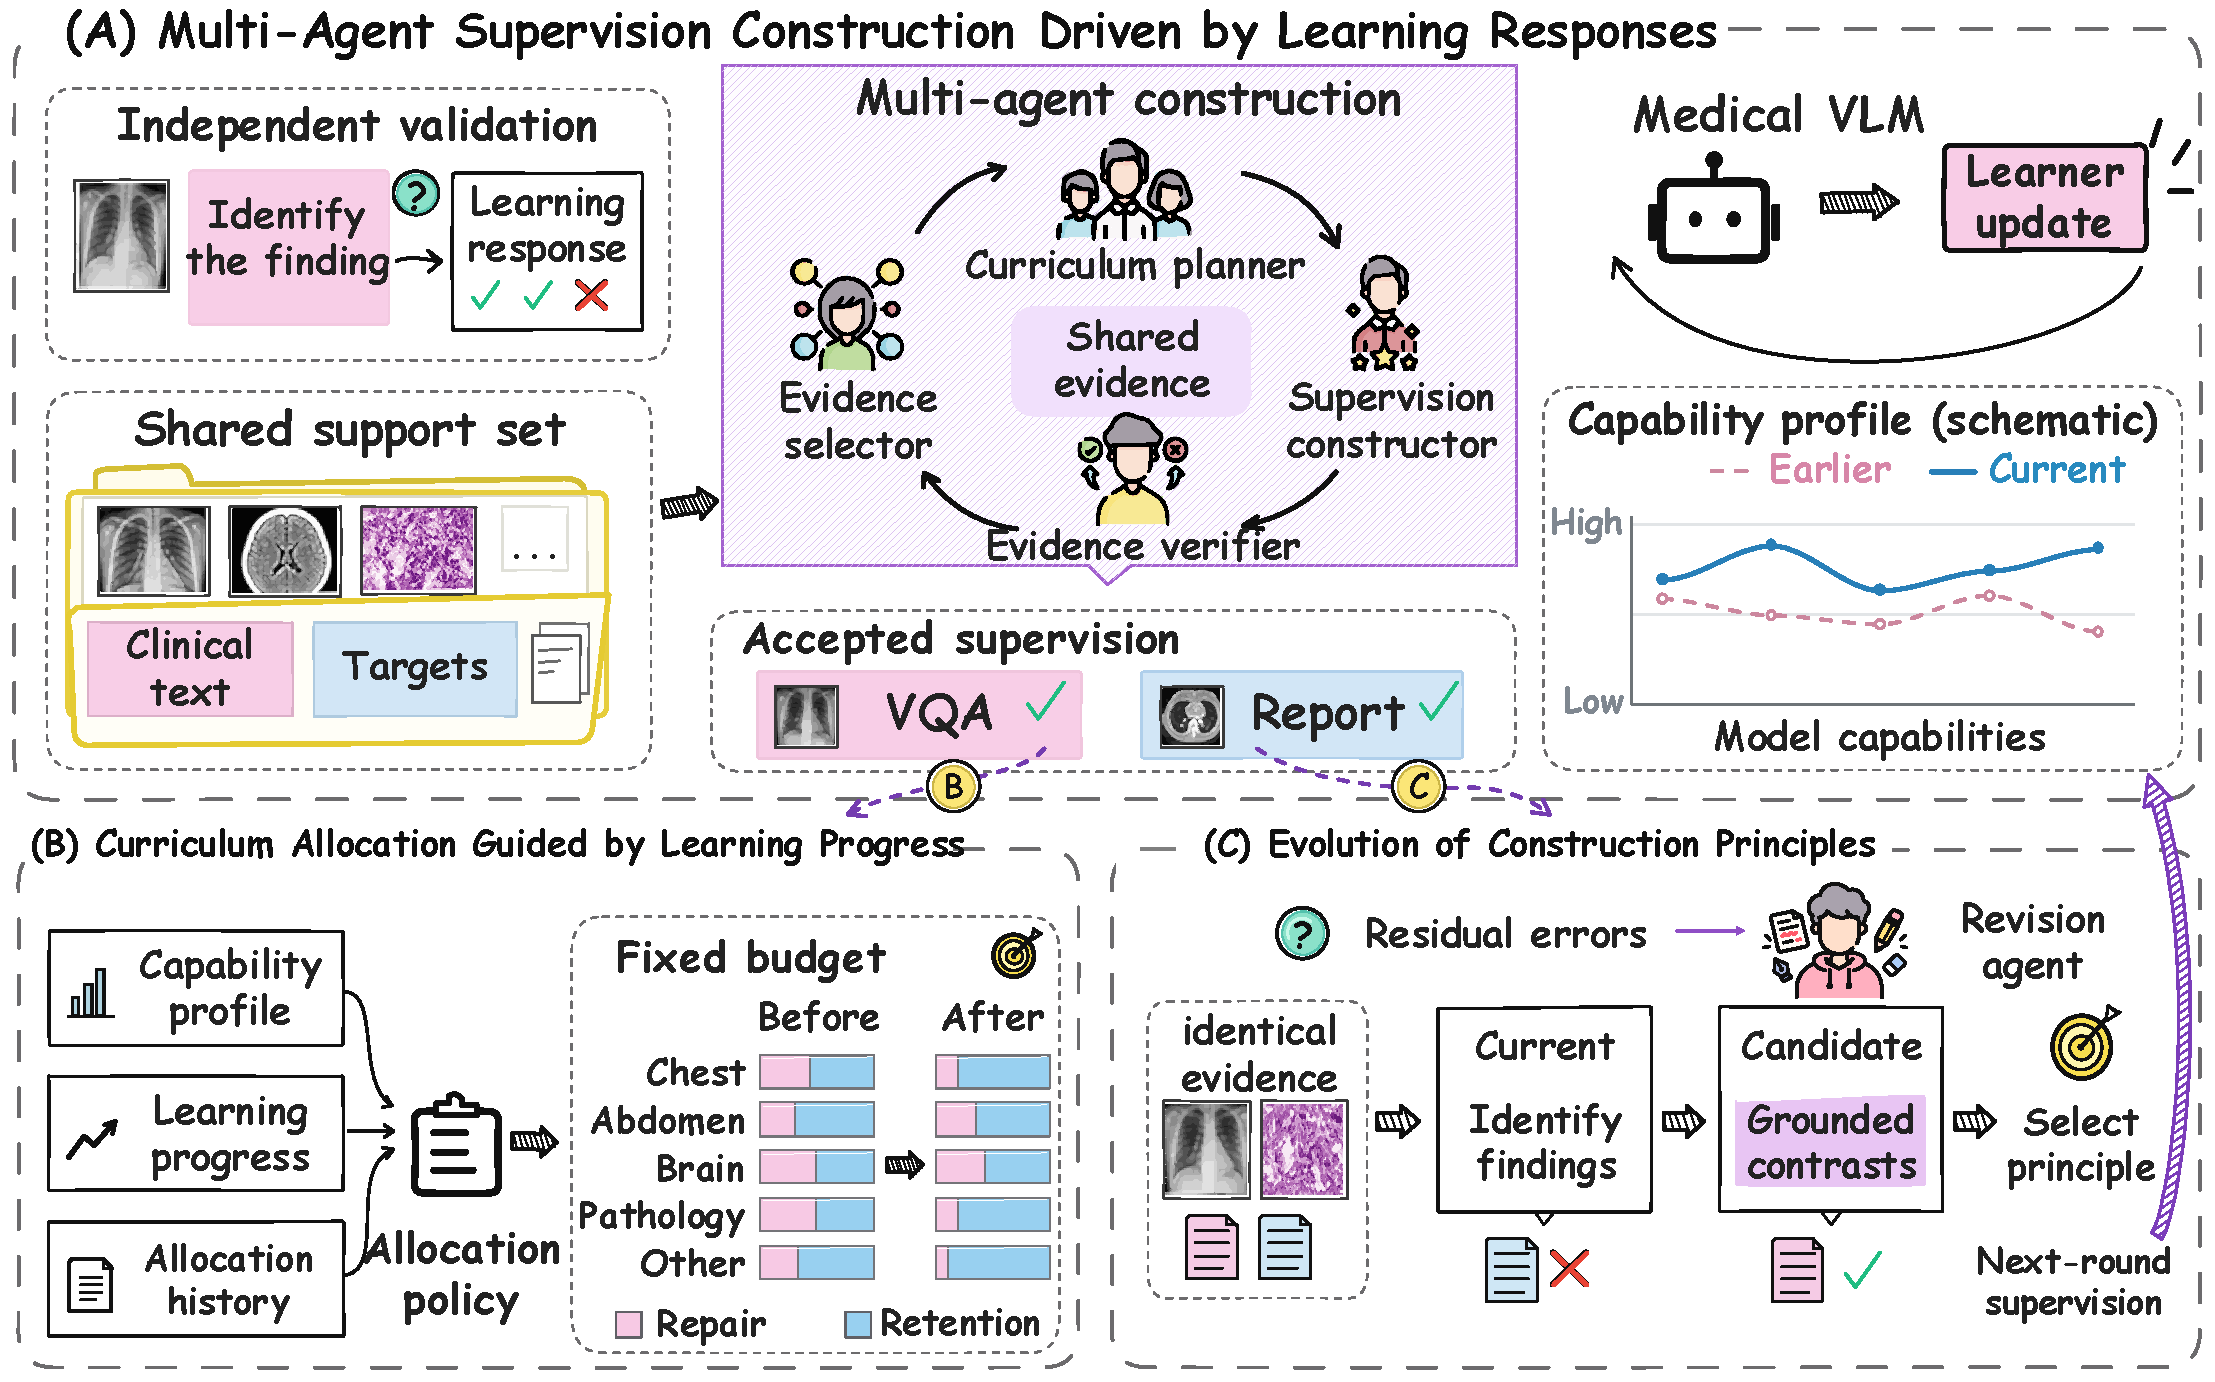
\includegraphics[width=\linewidth]{figures/evoforma_framework.pdf}
\caption{CoEvoMed 框架。（A）多智能体协作基于医学证据构造并验证监督，学习者更新后在独立任务验证集上产生学习响应。（B）学习进展指导固定任务预算下的课程分配。（C）修订智能体依据学习响应修订构造原则，比较当前原则与候选原则基于相同证据生成的监督；被接受的修订用于后续监督构造。}
\label{fig:framework}
\end{figure}
\endgroup

CoEvoMed 通过学习响应将监督构造与学习者更新联系起来（图~\ref{fig:framework}）。其多智能体系统结合课程分配与原则演化：课程分配决定构造投入，修订后的原则则改变智能体将医学证据组织为监督的方式。

\subsection{学习响应驱动的多智能体监督构造}
\label{sec:multiagent}

课程规划器依据能力反馈确定分配份额与构造目标。证据选择器从$\mathcal S$检索兼容的视觉记录与支持事实；监督构造器依据$\Sigma_e$形成问答对或报告，证据验证器检查事实一致性、视觉依赖、有效性与重复。接受的监督$\mathcal D_e^{\mathrm{syn}}$保留其证据来源与所用原则，用于后续评价。

% Queue Table 1 early to preserve its page-top placement.
\begin{table}[!t]
\centering\small
\caption{医学 VQA 准确率（\%）。粗体标识 CoEvoMed，其 8B 分数统一采用 R7 检查点。}
\label{tab:main}
\setlength{\tabcolsep}{4pt}
\renewcommand{\arraystretch}{1.05}
\begin{tabularx}{\linewidth}{@{}Y*{4}{>{\centering\arraybackslash}p{0.14\linewidth}}@{}}
\toprule
模型 & PMC-VQA & VQA-RAD & SLAKE & PathVQA\\
\MainResultsRows
\end{tabularx}
\end{table}

学习者在规定预算内最小化$\mathcal D_e^{\mathrm{mix}}$上的回答 token 负对数似然（附录~\ref{app:learner_objective}）。每次更新后，CoEvoMed 在相同任务验证样本上对齐相邻轮次的预测。能力单元$c$的观测增量为
\begin{equation}
\widehat{\Delta\kappa}_e(c)=\mathcal J_c[M_e]-\mathcal J_c[M_{e-1}],
\quad e\geq1.
\label{eq:capability_change}
\end{equation}
配对变化区分不足消解、能力回退与持续缺口，揭示净进展之外的修复与保持需求。摘要$\mathbf{s}_e$汇总当前掌握水平、能力变化及分配历史，以指导课程分配。响应中的残余错误反映能力与任务要求的差距，其语义指导构造目标与原则修订。

演化窗口由一组训练轮次组成，用于汇总原则使用情况与学习响应。每个窗口结束时，修订智能体依据残余错误提出候选原则，通过相同证据下的监督比较确定用于后续监督构造的修订（第~\ref{sec:strategy_evolution}节）。完整过程见附录~\ref{app:algorithm}。

\subsection{学习进展指导的课程分配}
\label{sec:curriculum}

课程规划器依据课程分配策略选择$a_e\sim\mu_{\theta_e}(\cdot\mid \mathbf{s}_e)$，平衡修复与保持，并决定是否聚焦错误证据最强的能力区域。修复针对较弱能力中的未解决缺口与新近回退，保持维持对已掌握能力的覆盖。分配映射$\mathcal A$将动作与历史证据转化为构造份额：
\begin{equation}
\boldsymbol q_e=\mathcal A(a_e,h_e),\qquad
\sum_{c\in\mathcal C_t}q_{e,c}=\bar q_t,
\label{eq:quota}
\end{equation}
其中，$\mathcal C_t$为任务$t$的能力单元集合，$\bar q_t$为预设任务份额。因此，适应在固定任务预算内重新配置投入。这些份额加权式~\ref{eq:supervision_mixture}中的候选分布，验证与混合进一步确定实际训练曝光。

以$U_t^{\mathrm{val}}$评价学习者在$\mathcal V_t$上的表现，令$\delta_{e,t}=U_t^{\mathrm{val}}(M_{e+1})-U_t^{\mathrm{val}}(M_e)$。奖励平衡 VQA 任务$\mathcal T_{\mathrm V}$与报告任务$\mathcal T_{\mathrm R}$：
\begin{equation}
r_e=G_e=\frac{1}{2|\mathcal T_{\mathrm V}|}\sum_{t\in\mathcal T_{\mathrm V}}\delta_{e,t}
+\frac{1}{2|\mathcal T_{\mathrm R}|}\sum_{t\in\mathcal T_{\mathrm R}}\delta_{e,t}.
\label{eq:gain}
\end{equation}
固定评价尺度使有符号奖励保留增益与回退。行为克隆初始化课程规划器，再以结合广义优势估计的 PPO，利用规划器与学习者之间的同策略交互优化式~\ref{eq:objective}~\citep{schulman2017proximal,schulman2016high}。混合策略与优化设置见附录~\ref{app:implementation}。

\subsection{构造原则的演化}
\label{sec:strategy_evolution}

课程分配调节不同能力上的构造投入，构造原则$\Sigma_e$则规定提问意图、证据与回答的关联及概念辨析，其适用性取决于学习者的能力状态。CoEvoMed 随学习需求的变化修订这些可复用原则。

每个窗口结束时，考虑修订使用充分且净修复不为正的原则；净修复为修复样本数减去回退样本数。残余错误的语义引导构造原则修订，同时保持目标能力与医学事实不变。例如，定位错误引导构造原则建立更明确的局部证据与目标回答之间的关联。

当前原则与候选原则在相同证据及匹配配额下分别构造监督。选择过程评价事实一致性与任务适配性，包括修订是否表达了目标证据关联、概念对比或事实覆盖。可用产出率（证据分配中产生可用监督的比例）与配对覆盖率（两种原则均产生可用监督的证据分配比例）作为筛选条件，具体阈值见附录~\ref{app:implementation}。

接受的修订作为生效构造原则持续保留~\citep{zhang2026agentic}。所得监督作用于学习者更新，新的验证响应继续引导原则修订：
\begin{equation}
\Sigma_{e+1}=\mathscr E(\Sigma_e,h_{e+1},\mathcal S).
\label{eq:strategy_evolution}
\end{equation}
其中，$h_{e+1}$包含学习者更新后的观测与奖励。演化窗口之间及候选未被接受时，算子保留对应的生效原则。

\section{实验}
\label{sec:experiments}

\subsection{评测设置}

2D 评测包括 VQA-RAD、SLAKE、PMC-VQA 和 PathVQA~\citep{lau2018dataset,liu2021slake,zhang2024pmc,he2020pathvqa}，以及 MIMIC-CXR 和 IU-Xray 报告生成~\citep{johnson2019mimic,demnerfushman2016preparing}；三维评测覆盖 M3D-VQA 闭合题、3D-RAD 开放题与 AMOS-MM 报告生成~\citep{bai2024m3d,gai2025threedrad,ji2024amosmm}。主要学习者为 Qwen3-VL-8B-Instruct~\citep{bai2025qwen3}，Gemma-3-4B-IT~\citep{gemmateam2025gemma}与 InternVL3-9B~\citep{zhu2025internvl3}用于跨架构验证，其中 InternVL3-9B 的实验结果见附录~\ref{app:internvl}。任务验证指导适应，支持证据用于监督构造，外部基准评价学习结果。

比较结合本研究评测与 Hulu-Med~\citep{jiang2025hulumed}、Lingshu~\citep{lasateam2025lingshu}、MedVLSynther-7B~\citep{huang2026synthesizing}及 CURE-4B~\citep{messina2026cure}的已发表结果。



\subsection{医学多模态性能}

CoEvoMed-8B 在四项 VQA 基准上较 Hulu-Med-7B 提高 1.15--4.80 个准确率百分点，CoEvoMed-32B 则在各项基准上均领先纳入比较的模型（表~\ref{tab:main}）。报告生成中，8B 在 IU-Xray 上达到 68.22，32B 在 MIMIC-CXR 上达到 64.33（图~\ref{fig:report_results}）。8B 的六项结果统一采用 R7 检查点，其在所考察轮次中实现了问答与报告生成能力的最佳整体平衡。

从相同的 Qwen3-VL-8B 初始化出发，CoEvoMed 使用更少的训练样本，在四项 VQA 基准上均优于使用约 70 万条原始数据直接训练的对照（附录~\ref{app:raw_source}）。这一比较支持自适应监督构造与课程配置在原始数据规模之外的性能贡献。



\begin{figure}[!htb]
\centering
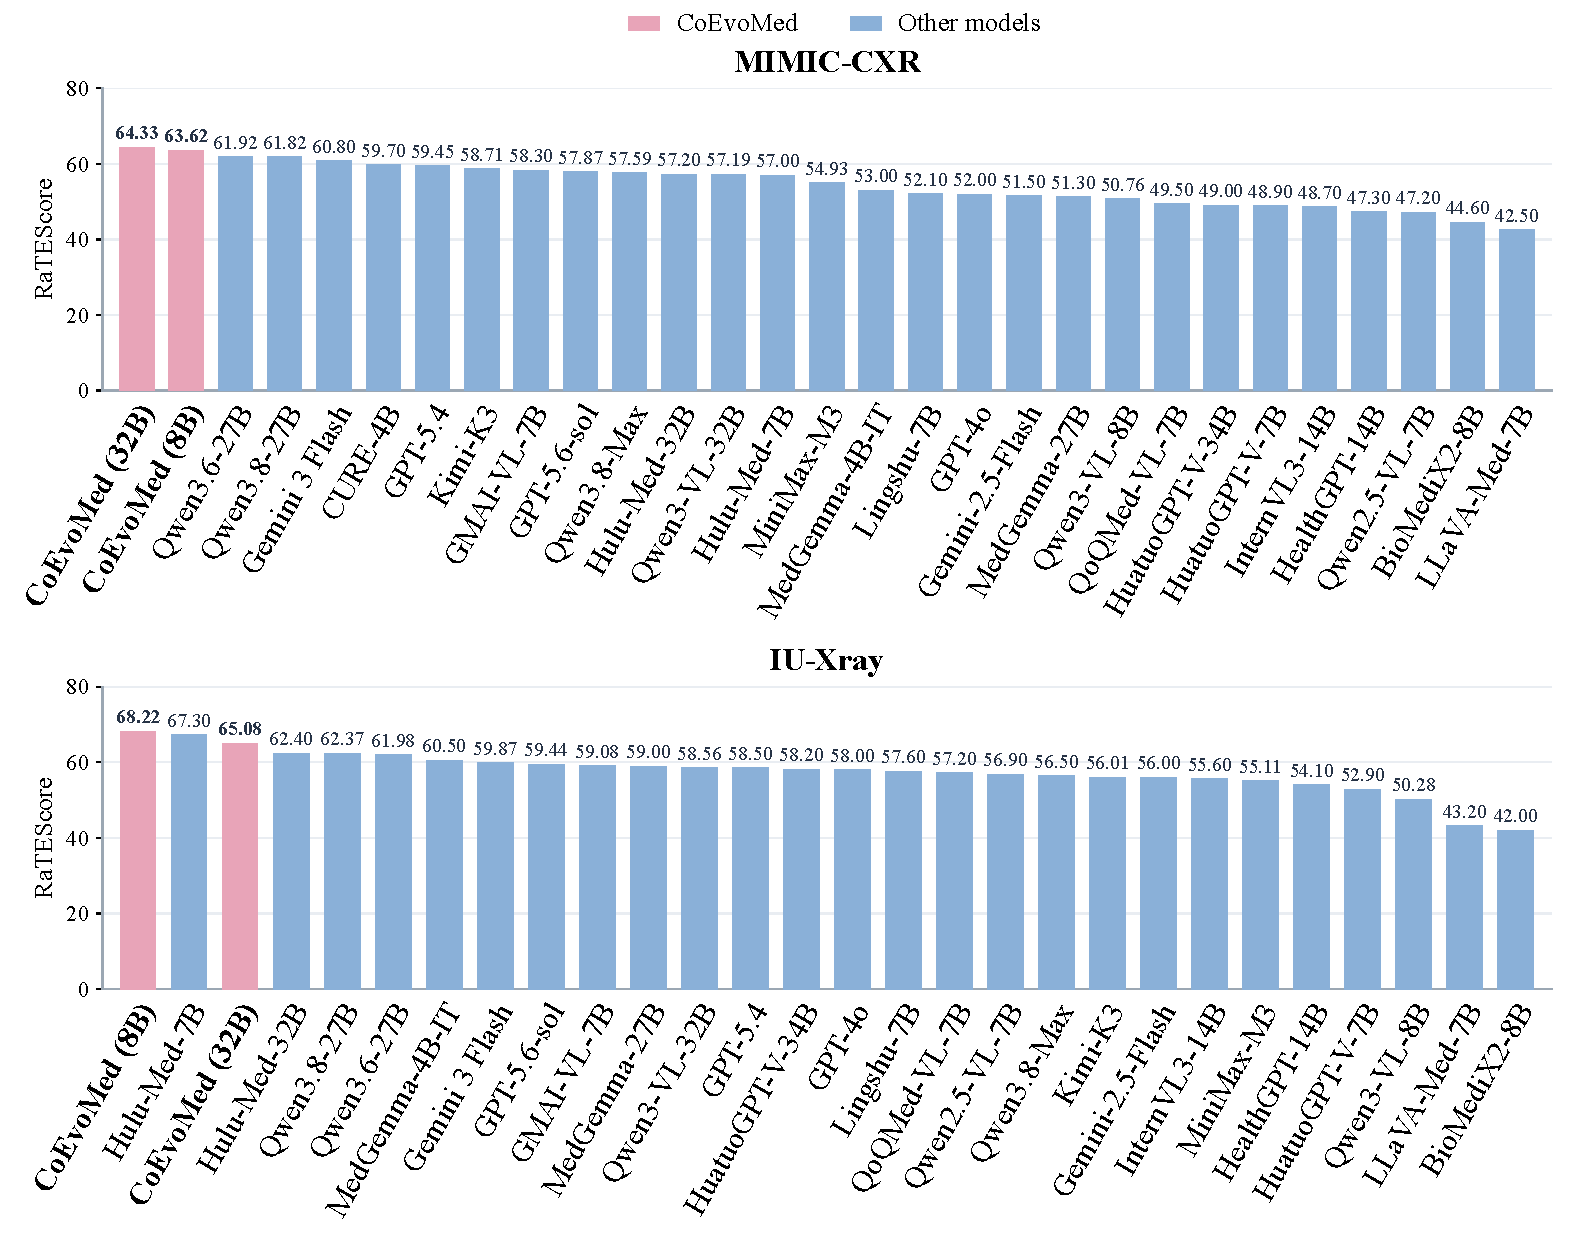
\includegraphics[width=0.90\linewidth,trim=0 14.8bp 0 4bp,clip]{figures/report_ratescore.pdf}
\caption{MIMIC-CXR（上，29个模型）与 IU-Xray（下，28个模型）的报告生成表现，分别按 RaTEScore（$\times100$）降序排列。粉色为 CoEvoMed，蓝色为基线。CURE-4B 采用 AGRG-29 + GRG 配置。补充指标见图~\ref{fig:report_lexical}。}
\label{fig:report_results}
\end{figure}

\paragraph{三维医学数据适用性。}
CoEvoMed 在图~\ref{fig:3d_main}的三项基准汇总比较中均位列首位，分别对应 M3D-VQA 宏平均准确率、3D-RAD 宏平均 ROUGE-1 与 AMOS-MM RaTEScore，将评价范围拓展至三维问答与报告生成。类别级结果、补充指标与评价协议见附录~\ref{app:3d}。

\begin{figure}[!htb]
\centering
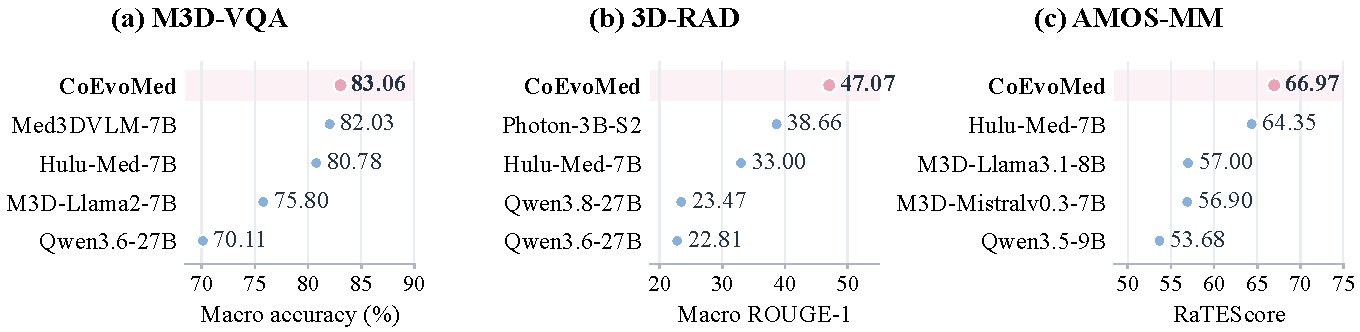
\includegraphics[width=\linewidth]{figures/three_d_main.pdf}
\caption{三维评测：（a）M3D-VQA 宏平均准确率；（b）3D-RAD 宏平均 ROUGE-1；（c）AMOS-MM RaTEScore，分数均乘以100。各面板展示 CoEvoMed（粉色），以及附录~\ref{app:3d}比较范围内按对应指标排名最高的四个基线（蓝色）。}
\label{fig:3d_main}
\end{figure}

\subsection{学习动态与机制分析}
\label{sec:analysis}
\label{sec:mechanisms}

我们考察学习轨迹、反馈与学习者状态的匹配性，以及构造原则效用的阶段依赖性。机制比较采用 VQA-RAD 与 MIMIC-CXR，完整结果与协议见附录~\ref{app:mechanisms}。

\paragraph{反馈与学习者状态的匹配性。}
各组从同一 R5 检查点出发，将数值能力统计与错误语义摘要共同替换为 R2、R3 或当前 R5 的验证反馈，指导课程分配与监督构造。当前反馈使 VQA-RAD 与 MIMIC-CXR 分别提高 2.62 个百分点与 2.77 分，均优于历史反馈（表~\ref{tab:ablations}，面板 A），支持课程适配与学习者当前能力状态及错误模式保持一致。

\paragraph{训练阶段依赖性。}
将原始与演化原则交叉应用于第2、5轮训练后的检查点（R2、R5），可观察到阶段依赖的监督效用（表~\ref{tab:ablations}，面板 B）。VQA-RAD 上，原始原则在 R2 领先 4.22 分，演化原则则在 R5 领先 8.26 分；MIMIC-CXR 上，演化原则的优势由 0.12 分扩大至 9.21 分。这种阶段依赖支持监督随学习者发展而修订，六项基准结果见附录~\ref{app:stage_transfer}。

\begin{table}[!htb]
\centering\small
\caption{机制消融：（A）R5 学习者的历史与当前反馈；（B）R2、R5 的原始与演化原则。VQA-RAD 为准确率（\%），MIMIC-CXR 为 RaTEScore（$\times100$）；参照为继续训练前分数。}
\label{tab:ablations}
\setlength{\tabcolsep}{3.5pt}
\renewcommand{\arraystretch}{1.08}
\begin{minipage}[t]{0.47\linewidth}
\vspace{0pt}
\begin{tabularx}{\linewidth}{Yrr}
\toprule
\multicolumn{3}{l}{\textbf{A. R5 学习者的反馈来源}}\\
\midrule
设置 & VQA-RAD & MIMIC-CXR\\
\midrule
R5：训练前 & 73.61 & 59.00\\
R2 反馈 & 72.51 & 59.11\\
R3 反馈 & 71.84 & 58.16\\
\rowcolor{mainOurs} \textbf{R5 反馈} & 76.23 & 61.77\\
\bottomrule
\end{tabularx}
\end{minipage}\hfill
\begin{minipage}[t]{0.50\linewidth}
\vspace{0pt}
\begin{tabularx}{\linewidth}{Yrr}
\toprule
\multicolumn{3}{l}{\textbf{B. 对训练阶段的依赖}}\\
\midrule
设置 & VQA-RAD & MIMIC-CXR\\
\midrule
R2：训练前 & 61.64 & 53.31\\
R2：原始原则 & 63.42 & 56.35\\
R2：演化原则 & 59.20 & 56.47\\
\midrule
R5：训练前 & 73.61 & 59.00\\
R5：原始原则 & 67.97 & 52.56\\
\rowcolor{mainOurs} \textbf{R5：演化原则} & 76.23 & 61.77\\
\bottomrule
\end{tabularx}
\end{minipage}
\end{table}

\paragraph{跨骨干适用性。}

Gemma-3-4B-IT 在 R7 达到 70.73\% 的 VQA 语义准确率与 65.89 的 MIMIC-CXR RaTEScore，较 Base 分别提高 22.39 和 16.23 分（图~\ref{fig:gemma_trajectory}）。同一检查点同时取得观测范围内并列最高的 VQA 准确率与最高报告分数，支持框架在更小规模、Qwen 家族之外的适用性。

\begin{figure}[!htb]
\centering
\vspace{-6pt}
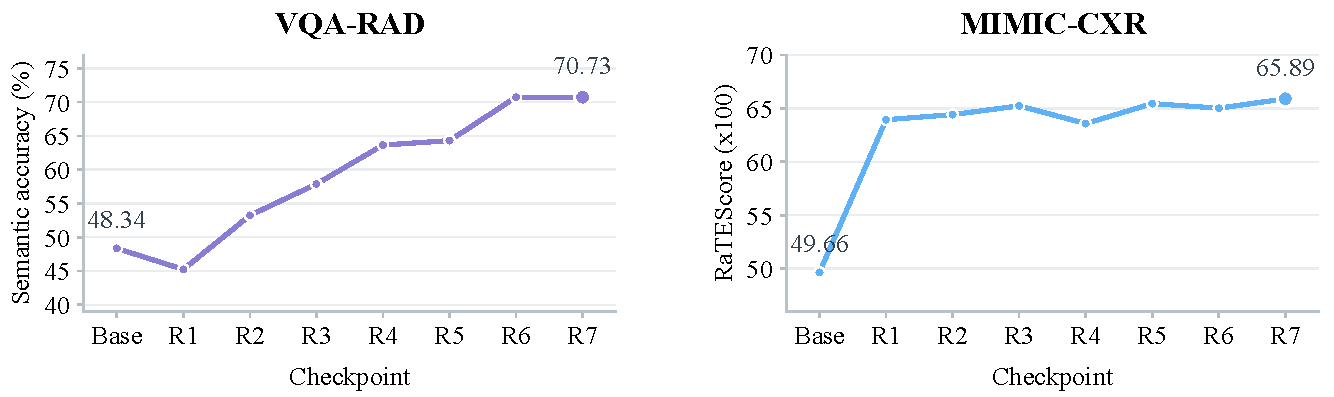
\includegraphics[width=0.85\linewidth]{figures/gemma_trajectory.pdf}
\caption{Gemma-3-4B-IT 从 Base 到 R7 的跨骨干验证。VQA-RAD 使用语义准确率（\%），MIMIC-CXR 使用乘以 100 的 RaTEScore。R7 的两项成绩来自同一 checkpoint。}
\label{fig:gemma_trajectory}
\end{figure}
\vspace{-10pt}
\begin{figure}[H]
\noindent\begin{minipage}[t]{0.40\textwidth}
\vspace{0pt}
\textbf{学习轨迹。} 图~\ref{fig:task_qa}显示，R1--R6 中属性问答提升、器官识别趋稳，定位问答在回落后恢复。这些分化的轨迹表明，不同任务的能力发展并不同步，为构造原则修订与构造分配提供状态信息。图~\ref{fig:trajectory}显示 SLAKE、PathVQA 与 IU-Xray 整体提升，并在 R7--R8 达到观测峰值。两组结果将学习者响应与外部基准性能联系起来，分别刻画能力发展及其在独立外部基准上的表现。
\end{minipage}\hfill
\begin{minipage}[t]{0.56\textwidth}
\vspace{0pt}\centering
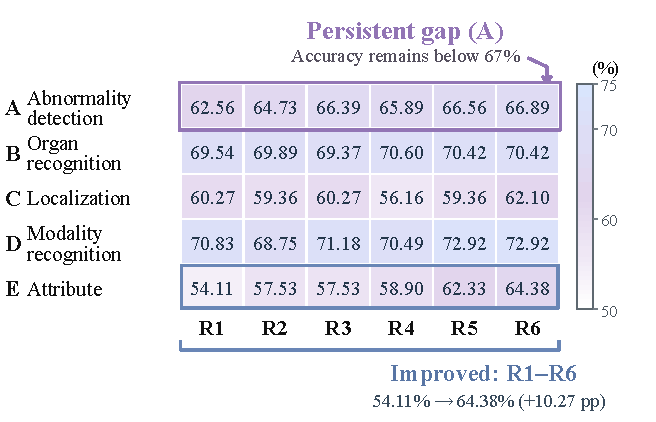
\includegraphics[width=\linewidth]{figures/task_qa_heatmap.pdf}
\caption{Qwen3-VL-8B 学习者在完成 R1--R6 训练后，于验证集上五类选定问答任务的准确率（\%）。}
\label{fig:task_qa}
\end{minipage}
\end{figure}
\vspace{-10pt}
\begin{figure}[H]
\centering
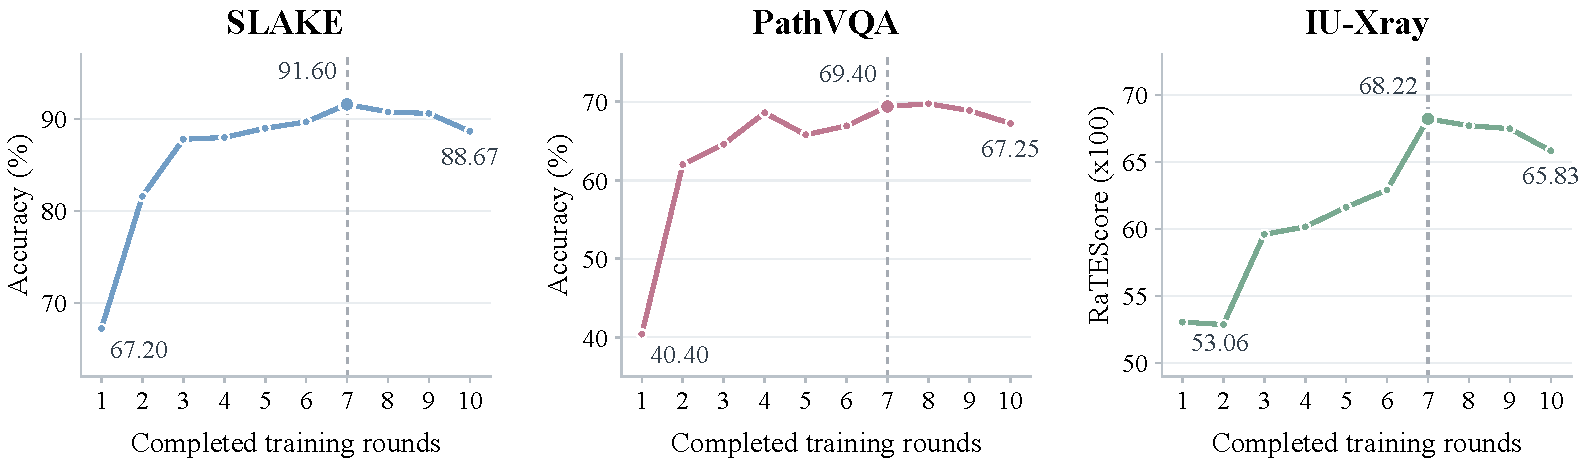
\includegraphics[width=0.85\linewidth]{figures/evolution_trajectory.pdf}
\caption{CoEvoMed-8B 的学习轨迹。虚线标记六项二维主结果统一采用的 R7 检查点。}
\label{fig:trajectory}
\end{figure}
\vspace{-12pt}
\FloatBarrier
\section{结论}
\label{sec:conclusion}

CoEvoMed 将监督构造视为医学视觉语言学习中持续演化的组成部分。构造原则随学习者的任务能力变化而修订，由此形成的监督进一步塑造后续能力发展。课程分配依据观测到的学习进展配置固定构造预算，与原则演化相互配合。多智能体协作将这两类适应过程结合起来，以医学证据为基础，使监督内容及其分配共同随学习者发展而调整。

二维视觉问答、报告生成、三维任务及不同骨干模型上的实验支持了该框架的有效性。不同反馈来源与训练阶段的比较进一步表明，使监督构造与学习者当前能力状态相匹配能够提高其效用。这些发现表明，监督构造方式与构造投入分配的协同调整，有助于提升医学多模态学习的效果。
